% 
% Originally from Jeff Philips, University of Utah
%
\documentclass[11pt]{article}

\usepackage{euscript}
\usepackage{amsmath}
\usepackage{amsthm}
\usepackage{amssymb}
\usepackage{epsfig}
\usepackage{xspace}
\usepackage{color}
\usepackage{url}
\usepackage{graphicx}
\usepackage{subcaption}
\usepackage{float}
\usepackage[utf8]{inputenc}
\usepackage[english]{babel}
\usepackage{fancyhdr}
\usepackage{graphicx}
\usepackage{subcaption}
\usepackage{float}

%\usepackage{wrapfig}



%%%%%%%  For drawing trees  %%%%%%%%%
%\usepackage{tikz}
%\usetikzlibrary{calc, shapes, backgrounds}
%%%%%%%%%%%%%%%%%%%%%%%%%%%%%%%%%
\setlength{\textheight}{9in}
\setlength{\topmargin}{-0.600in}
\setlength{\headheight}{0.2in}
\setlength{\headsep}{0.250in}
\setlength{\footskip}{0.5in}
\flushbottom
\setlength{\textwidth}{6.5in}
\setlength{\oddsidemargin}{0in}
\setlength{\evensidemargin}{0in}
\setlength{\columnsep}{2pc}
\setlength{\parindent}{1em}
%%%%%%%%%%%%%%%%%%%%%%%%%%%%%%%%%


\newcommand{\eps}{\varepsilon}
%\newfloatcommand{capbtabbox}{table}[][\FBwidth]
\renewcommand{\c}[1]{\ensuremath{\EuScript{#1}}}
\renewcommand{\b}[1]{\ensuremath{\mathbb{#1}}}
\newcommand{\s}[1]{\textsf{#1}}
\graphicspath{{plots/}}
\newcommand{\E}{\textbf{\textsf{E}}}
\renewcommand{\Pr}{\textbf{\textsf{Pr}}}

\title{Project 2 Report
\footnote{\s{EE 239AS ; Winter 2016 }
}
}
\author{Tushar Sudhakar Jee, Shubham Agarwal, Pulkit Aggarwal, Ishan Upadhyaya
	}


\begin{document}
\maketitle


\section{Dataset and Problem Statement}
\subsection{Part A}
Number of documents in Recreational Activity are 2389 and number of documents in Computer Technology are 2343\\

\begin{figure}[h]
	\centering
	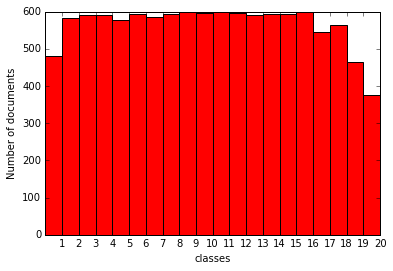
\includegraphics[scale = 0.5]{histogram.png}
	\caption{Histogram for the number of documents}
\end{figure}

\newpage
\section{Modeling Text Data and Feature Extraction}
\subsection{Part B}
Final number of terms extracted are 34792.

\subsection{Part C}
Ten Most significant features with TFICF 
scores are shown in Table \ref{table:si_wo} \\
\begin{table}[h]
	\centering
	\begin{tabular}{|c|c|c|c|c|} \hline
		Index & comp.sys.ibm.pc.hardware & comp.sys.max.hardware & misc.forsale & soc.religion.christian\\ \hline
		1 & scsi & mac & dos & god \\
		2 & drive & use & new & christian\\ 
		3 & use & scsi & sale & jesus \\
		4 & mb & appl & offer & church \\
		5 & ide & drive & use & christ \\
		6 & card & mb & includ & peopl \\
		7 & disk & simm & ship & say \\
		8 & control & problem & price & bibl \\
		9 & dos & quadra & wolverin & believ \\
		10 & jumper & nubus & sell & think \\
		\hline
	\end{tabular}
	\caption{Ten most significant words.}
	\label{table:si_wo}
\end{table}

\section{Feature Selection}
\subsection{Part D}
On applying LSI to the TFIDF matrix with k = 50, each document was mapped to a 50 dimensional vector. 

\newpage
\section{Learning Algorithms}

\subsection{Part E: Linear SVM}
The ROC curve for Linear SVM is shown below.

\begin{figure}[H]
	\centering
	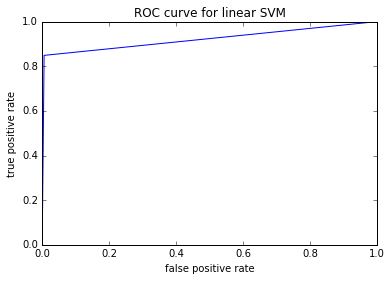
\includegraphics[scale = 0.6]{ROC_SVM.png}
	\caption{ROC curve for linear SVM}
\end{figure}

The confusion matrix for Linear SVM is shown below.
\begin{table}[H]
	\centering
	\begin{tabular}{|c|c|c|c|} \hline
		& Predicted Computer Technology & Predicted Recreation Activity \\ \hline
		Actual Computer Technology & 1581 & 9 \\
		Actual Recreation Activity & 236& 1324  \\
		\hline
	\end{tabular}
	\caption{Confusion Matrix: Linear SVM}
\end{table}


Accuracy, Precision and Recall for Linear SVM are shown below
\begin{table}[H]
	\centering
	\begin{tabular}{|c|c|c|c|} \hline
		Learning Algorithm & Accuracy & Precision & Recall\\ \hline
		Linear SVM & 92.22 & 99.32 & 84.87 \\
		\hline
	\end{tabular}
	\caption{Liner SVM}
\end{table}


\newpage
\subsection{Part F: Soft Margin SVM}

The ROC curve for Soft Margin SVM is shown below.

\begin{figure}[H]
	\centering
	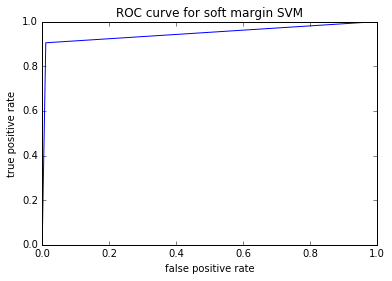
\includegraphics[scale = 0.6]{ROC_SMSVM.png}
	\caption{ROC curve for Soft Margin SVM}
\end{figure}

The confusion matrix for Soft Margin SVM is shown below.

\begin{table}[H]
	\centering
	\begin{tabular}{|c|c|c|c|} \hline
		& Predicted Computer Technology & Predicted Recreation Activity \\ \hline
		Actual Computer Technology & 1573 & 17 \\
		Actual Recreation Activity & 148& 1412  \\
		\hline
	\end{tabular}
	\caption{Confusion Matrix: Soft Margin SVM}
\end{table}

Accuracy, Precision and Recall for Soft Margin SVM are shown below

\begin{table}[H]
	\centering
	\begin{tabular}{|c|c|c|c|} \hline
		Learning Algorithm & Accuracy & Precision & Recall\\ \hline
		Soft margin SVM & 94.76 & 98.81 & 90.51 \\
		\hline
	\end{tabular}
	\caption{Soft Margin SVM}
\end{table}

\newpage
\subsection{Part G Naive Bayes}

The ROC curve for Naive Bayes is shown below.

\begin{figure}[H]
	\centering
	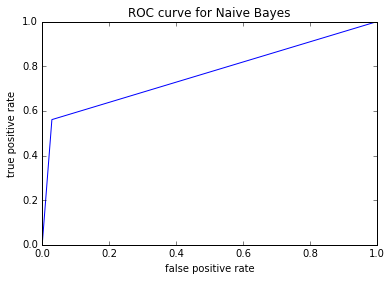
\includegraphics[scale = 0.6]{ROC_NaiveBayes.png}
	\caption{ROC curve for Naive Bayes}
\end{figure}

The confusion matrix for Naive Bayes is shown below.

\begin{table}[H]
	\centering
	\begin{tabular}{|c|c|c|c|} \hline
		& Predicted Computer Technology & Predicted Recreation Activity \\ \hline
		Actual Computer Technology & 1544 & 46 \\
		Actual Recreation Activity & 685& 875  \\
		\hline
	\end{tabular}
	\caption{Confusion Matrix: Naive Bayes}
\end{table}

Accuracy, Precision and Recall for Naive Bayes are shown below

\begin{table}[H]
	\centering
	\begin{tabular}{|c|c|c|c|} \hline
		Learning Algorithm & Accuracy & Precision & Recall\\ \hline
		Gaussian Naive Bayes& 76.79 & 95.00 & 56.08 \\
		\hline
	\end{tabular}
	\caption{Naive Bayes}
\end{table}

\newpage
\subsection{Part H Logistic Regression}

ROC curve for Logistic Regression is shown below

\begin{figure}[H]
	\centering
	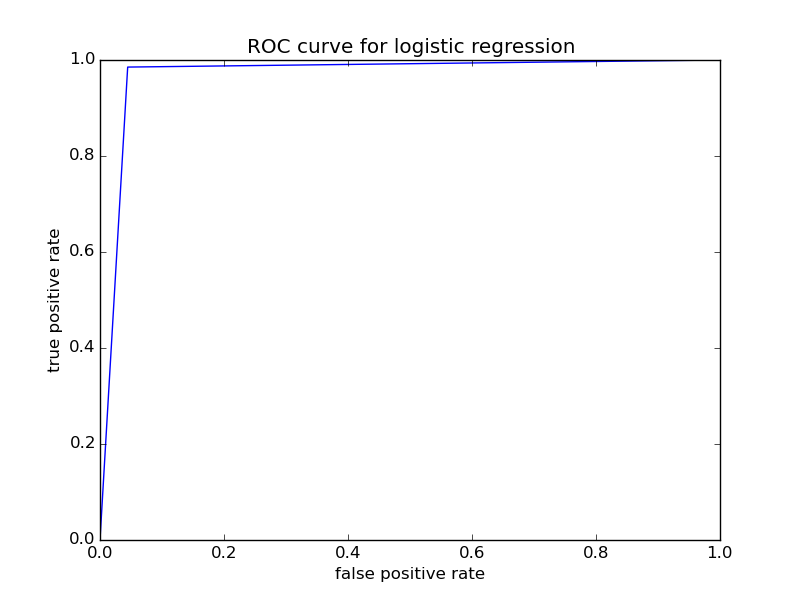
\includegraphics[scale = 0.6]{ROC_LogisticRegression.png}
	\caption{ROC curve for Logistic Regression}
\end{figure}

The confusion matrix for Logistic Regression is shown below.

\begin{table}[H]
	\centering
	\begin{tabular}{|c|c|c|c|} \hline
		& Accuracy 		Predicted Computer Technology & Predicted Recreation Activity \\ \hline
		Actual Computer Technology & 1519 & 71 \\
		Actual Recreation Activity & 23& 1537  \\
		\hline
	\end{tabular}
	\caption{Confusion Matrix: Logistic Regression}
\end{table}

Accuracy, Precision and Recall for Logistic Regression are shown below

\begin{table}[H]
	\centering
	\begin{tabular}{|c|c|c|c|} \hline
		Learning Algorithm & Accuracy & Precision & Recall\\ \hline
		Logistic Regression& 97.01 & 95.58 & 98.52 \\
		\hline
	\end{tabular}
	\caption{Logistic Regression}
\end{table}


\newpage
\section{Multi-class Classification}
\subsection{Part I}

The results for Multi-class classification are shown in the tables below. Table \ref{table:ovr_res} contains the results for One vs Rest method and Table \ref{table:ovo_res} contains the results for One vs One method.

\begin{table}[h]
	\centering
	\begin{tabular}{|c|c|c|c|} \hline
		Learning Algorithm & Accuracy & Precision & Recall\\ \hline
		Gaussian Naive Bayes & 63.32 & 64.50 & 63.32 \\
		Linear SVM & 81.40 & 81.50 & 81.40 \\
		\hline
		\end{tabular}
		\caption{One vs Rest}
		\label{table:ovr_res}
\end{table}

\begin{table}[h]
	\centering
	\begin{tabular}{|c|c|c|c|} \hline
		Learning Algorithm & Accuracy & Precision & Recall\\ \hline
		Gaussian Naive Bayes & 64.53 & 65.47 & 64.53 \\
		Linear SVM & 80.89 & 81.28 & 80.89 \\
		\hline
	\end{tabular}
	\caption{One vs One}
	\label{table:ovo_res}
\end{table}

The confusion matrix for One vs One methods are shown below in figure \ref{fig:cm_ovo} and Confusion matrix for One vs Rest methods are in figure \ref{fig:cm_ovr}

\begin{figure}[H]
	
	\begin{subfigure}[b]{0.5\textwidth}
		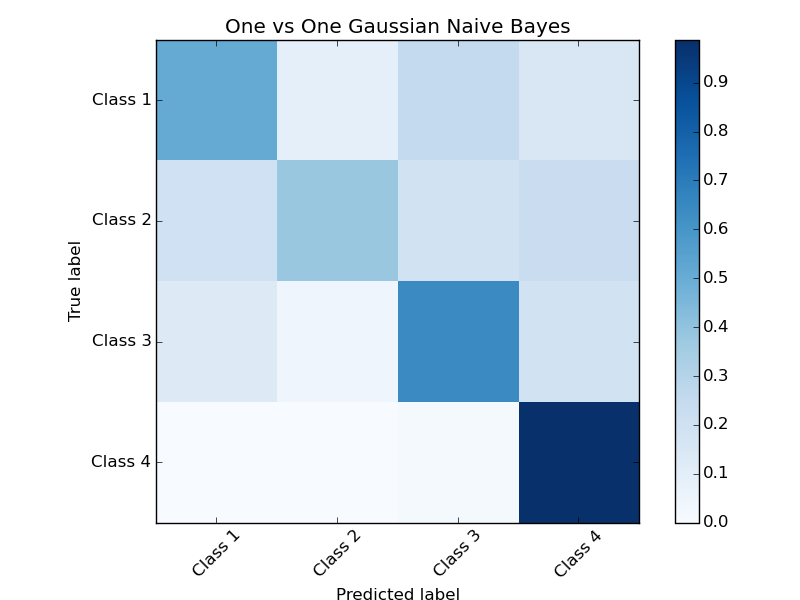
\includegraphics[width=\textwidth]{ovo_gnb.png}
		\caption{Gaussian Naive Bayes}
	\end{subfigure}
	%
	\begin{subfigure}[b]{0.5\textwidth}
		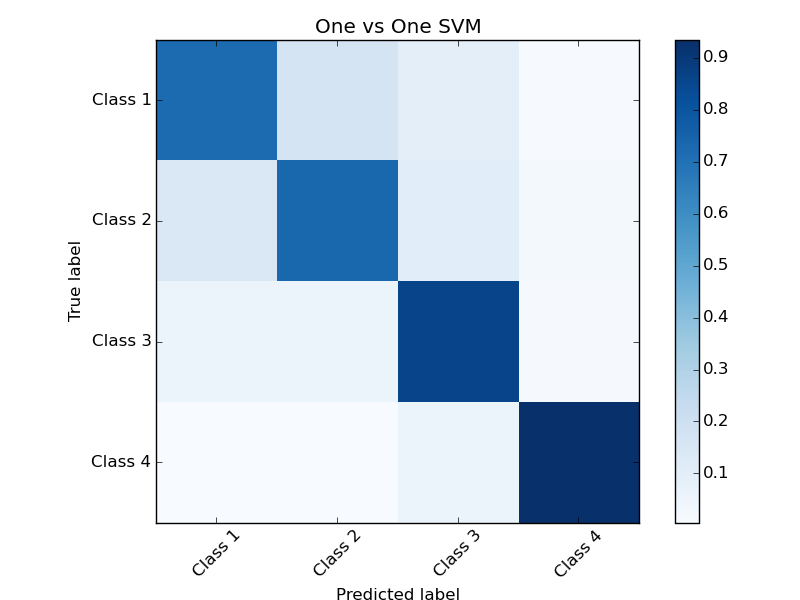
\includegraphics[width=\textwidth]{ovo_svm.png}
		\caption{Linear SVM}
	\end{subfigure}
	\caption{Confusion Matrix for One vs One Method}
	\label{fig:cm_ovo}
\end{figure}

\begin{figure}[H]
	
	\begin{subfigure}[b]{0.5\textwidth}
		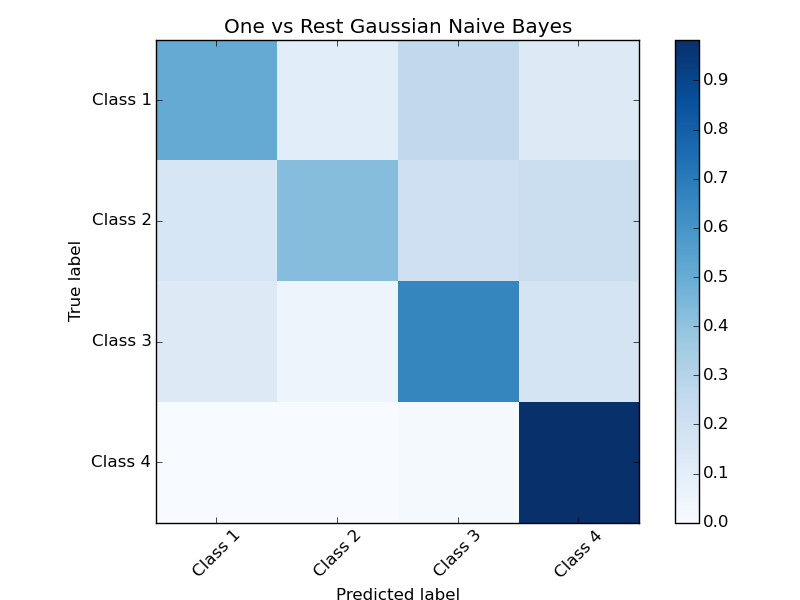
\includegraphics[width=\textwidth]{ovr_gnb.png}
		\caption{Gaussian Naive Bayes}
	\end{subfigure}
	%
	\begin{subfigure}[b]{0.5\textwidth}
		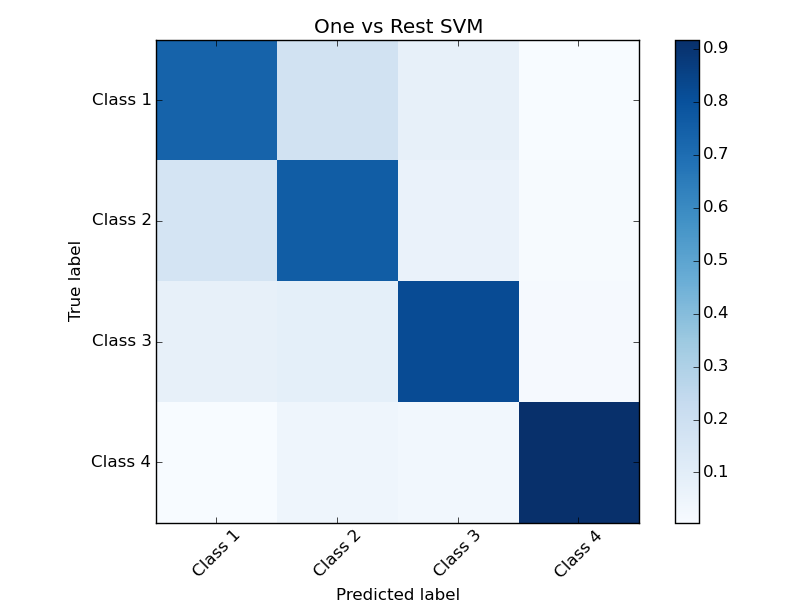
\includegraphics[width=\textwidth]{ovr_svm.png}
		\caption{Linear SVM}
	\end{subfigure}
	\caption{Confusion Matrix for One vs Rest Method}
	\label{fig:cm_ovr}
\end{figure}

\end{document}